%% a little excursion about trees

\section{the Barnes \& Hut tree algorithm}
In the previous chapter we saw a general formalism on how a cluster of particles can be approximated by multipole moments relative to their center of mass. This formalism however does not propose how to partition a given set of particles into clusters and clusters of clusters. The \emph{Barnes \& Hut tree algorithm} proposed in \cite{1986Natur.324..446B} does exactly that with the help a tree, a datastructure well suited to imply a hierarchy on a set of elements, in this case particles and clusters.

\subsection{A little excursion about trees}
First we need to know a few basic things about trees. A graph is a set of elements represented by \emph{nodes}. A tree is a rooted, directed graph in which any two nodes are connected by one and only one path. This means a node is the \emph{root node} and the connections between the nodes have a direction. Each node can have a number of children\footnote{often the term \emph{daughter} is used, but because of the asexual nature of tree nodes we are using here the term \emph{child}} 
nodes and has exactly one parent, expect for the root node which has no parent. Nodes can be assigned a depth. The root node per definition has depth $0$ and the children of a node have the inherit the depth of the parent increased by one. Figure \ref{fig:simpletree} shows a simple tree. The blue square represents the root node and has two children with depth 1, while on of this children has again two children with depth 2. Tree data structures are usually drawn upside-down, this means with the root on top and increasing depth to the bottom.

\begin{figure}[htbp]
\begin{center}
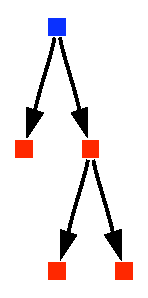
\includegraphics{simpletree.pdf}
\caption{A simple tree. the squares represent nodes which are interconnected by arrows pointing from the parent node to its children}
\label{fig:simpletree}
\end{center}
\end{figure}

Nodes without children are called \emph{leaf nodes}. A disjoint set of trees is called a \emph{forest}. One notices that the definition for a tree does not only fit the whole set of nodes of a tree, but also subsets. Every node can be taken as a root node and forms again a tree, also called a \emph{subtree} of the tree. Or one can say, that the children of a node form a forest of trees.

\subsection{Tree walks}
A tree walk is a sequence going through all the nodes of a tree once. For a tree with $N$ nodes there exist $N!$ possible tree walks, a few of them are special which are useful for the Barnes \& Hut tree algorithm.

\begin{figure}[htbp]
\begin{center}
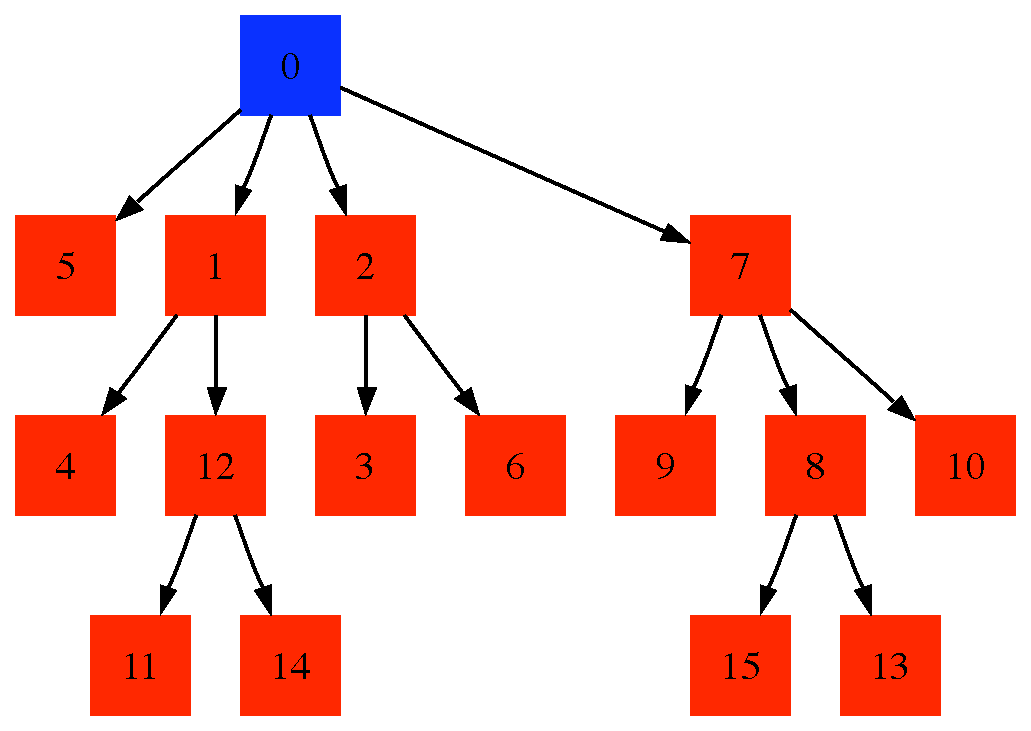
\includegraphics[scale=0.4]{simple_numbered_tree.pdf}
\caption{A slightly more complex tree with arbitrarly numbered nodes.}
\label{fig:simplenumtree}
\end{center}
\end{figure}

\paragraph{post order}
The post order tree walk starts at the root node. It can be implemented as shown in the following recursive algorithm
\begin{algorithm}
\caption{post order walk}
\begin{algorithmic}
\label{alg:postorder}
\STATE{pick current node}
\FORALL{children}
\STATE{go to child}
\STATE{do post order walk}
\ENDFOR
\end{algorithmic}
\end{algorithm}
\\

When $f_{post} (n)$ stands for applying the post order algorithm to node $n$ and the children are iterated from left to rigth, then the post order walk for the tree in figure \ref{fig:simplenumtree} can be elaborated in the following way
\begin{align}
\big\{& f_{post} (0) \big\} \nonumber \\
\big\{& 0, f_{post} (5),  f_{post} (1),  f_{post} (2),  f_{post} (7) \big\} \nonumber \\
\big\{& 0, 5, 1, f_{post} (4), f_{post} (12), 2, f_{post} (3), f_{post} (6), 7, f_{post} (9), f_{post} (8), f_{post} (10)\big\} \nonumber \\
\big\{& 0, 5, 1, 4, 12, f_{post} (11), f_{post} (14), 2, 3, 6, 7, 9, 8, f_{post} (15), f_{post} (13), 10 \big\} \nonumber \\
\big\{& 0, 5, 1, 4, 12, 11, 14, 2, 3, 6, 7, 9, 8, 15, 13, 10 \big\} \nonumber 
\end{align}

The key property of this walk is, that a node is not walked by unless every node on the path between the node and the root node has been walked. This property is useful, if a calculation on a node depends on results from the parent node.

\paragraph{pre order}
The pre order walk is similar to the post order walk, the only difference is that the children are walked before picking the current node. This gives the algorithm

\begin{algorithm}
\caption{pre order walk}
\begin{algorithmic}
\label{alg:preorder}
\FORALL{children}
\STATE{go to child}
\STATE{do pre order walk}
\ENDFOR
\STATE{pick current node}
\end{algorithmic}
\end{algorithm}

When $f_{post} (n)$ stands for applying the post order algorithm to node $n$, then the post order walk for the tree in figure \ref{fig:simplenumtree} can be elaborated in the following way

 %f_{post} ()
\begin{align}
\big\{& f_{pre} (0) \big\} \nonumber \\
\big\{& f_{pre} (5),  f_{pre} (1),  f_{pre} (2),  f_{pre} (7), 0\big\} \nonumber \\
\big\{& 5, f_{pre} (4), f_{pre} (12), 1,  f_{pre} (3),  f_{pre} (6), 2,  f_{pre} (9),  f_{pre} (8), f_{pre} (10), 7, 0\big\} \nonumber \\
\big\{& 5, 4,  f_{pre} (11),  f_{pre} (14), 12, 1, 3, 6, 2, 9,  f_{pre} (15),  f_{pre} (13), 8, 10, 7, 0\big\} \nonumber \\
\big\{& 5, 4, 11, 14, 12, 1, 3, 6, 2, 9, 15, 13, 8, 10, 7, 0\big\} \nonumber
\end{align}

The key property of the pre order walk, is that a node is not walked until all its children and their subtrees have been walked. Again, this is useful, if a calculation on a node depends on results from the children nodes.

\subsection{Trees for spatial subdivision}
A tree datastructure can be used to recursively subdivide space. The basic idea is to take a volume, assign this volume to a node in a tree, then subdivide this volume in disjoint subvolumes and assign these subvolumes to the children of the node. So the subdivision of space can be mapped onto a tree.\ The easiest form of subdivision is using volumes aligned with the dimensions and having the same side length in each dimension. So in 2D this corresponds to squares and in 3D to cubes along the axis. This volumes are then divided along each dimension into two equal-length intervals, which leads to $2^d$ subvolumes in $d$ dimensions. So if we have an arbitrary volume with a minimum $x_{i,min}$ and a maximum $x_{i,max}$ in each coordinate $i$ we can enclose this volume with a volume with sidelength $l$ and the center $x_{i,c}$

\begin{equation}
l = \max_{i} ( x_{i,max} - x_{i,min})  ~~~~ x_{i,center}= \frac{ x_{i,min} + x_{i,max} }{2}
\end{equation}

The $2^{d}$ subvolumes indexed with $j$ have a side length of $\frac{l}{2}$ and center vector components $i = 0 \dots d$, where $d_{i}$ stands for $i^{th}$ digit of the binary representation of the subvolume index $j$

\begin{equation}
x_{i, j~center} = x_{i,center} + l \frac{(-1)^{d_{i} + 1}}{2} ~~~~~ d_{i} = \frac{j  - \sum_{k \ne i} ( j \mod 2^{k} )}{2^{i}}
\end{equation}

In 2D this subvolumes are called \emph{quadrants}, in 3D \emph{octants}. The corresponding trees to which this subdivision can be mapped to are called \emph{quadtrees} and \emph{octrees}, having up to 4 and 8 children per node.

\subsection{the B\&H algorithm}
The Barnes \& Hut algorithm described in \cite{1986Natur.324..446B} subdivides the computational universe containing $N$ gravitationally interacting particles in subvolumes, called \emph{cells}. The particles are children of cell nodes. The tree must be built in a way, such that no cell octant contains more than one particle. An example of such a tree is shown in figure \ref{2D_CHtree} for 50 randomly distrbuted particles in 2D. 

\begin{figure}[htbp]
\begin{center}
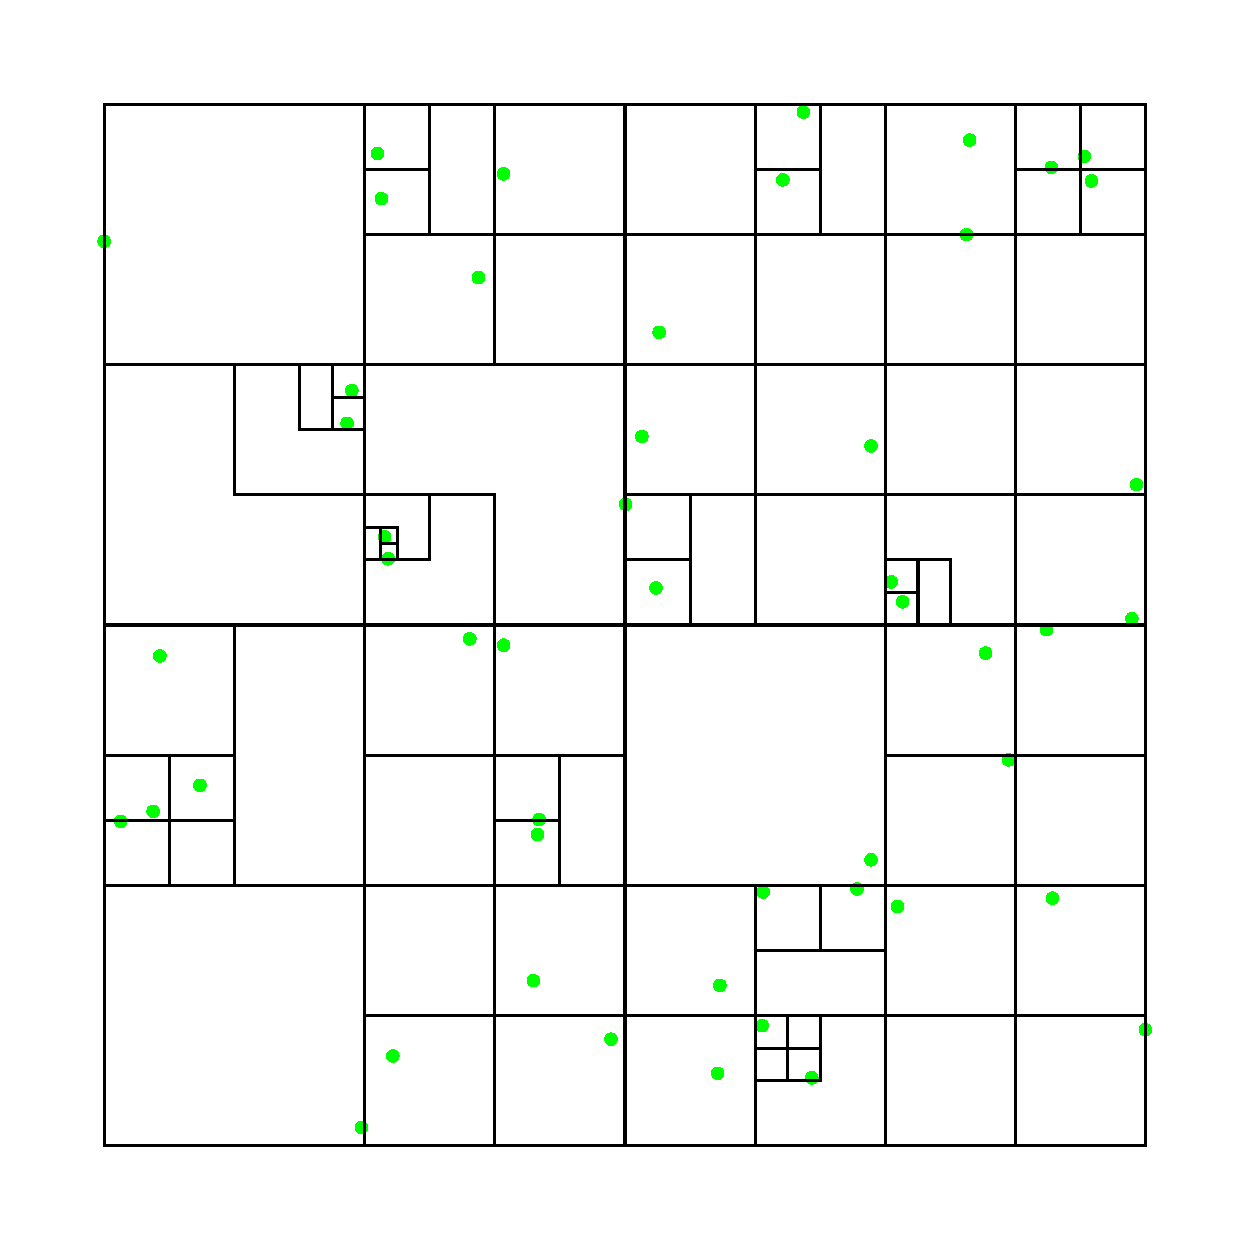
\includegraphics[scale=0.6]{quadtree50_xy.pdf}
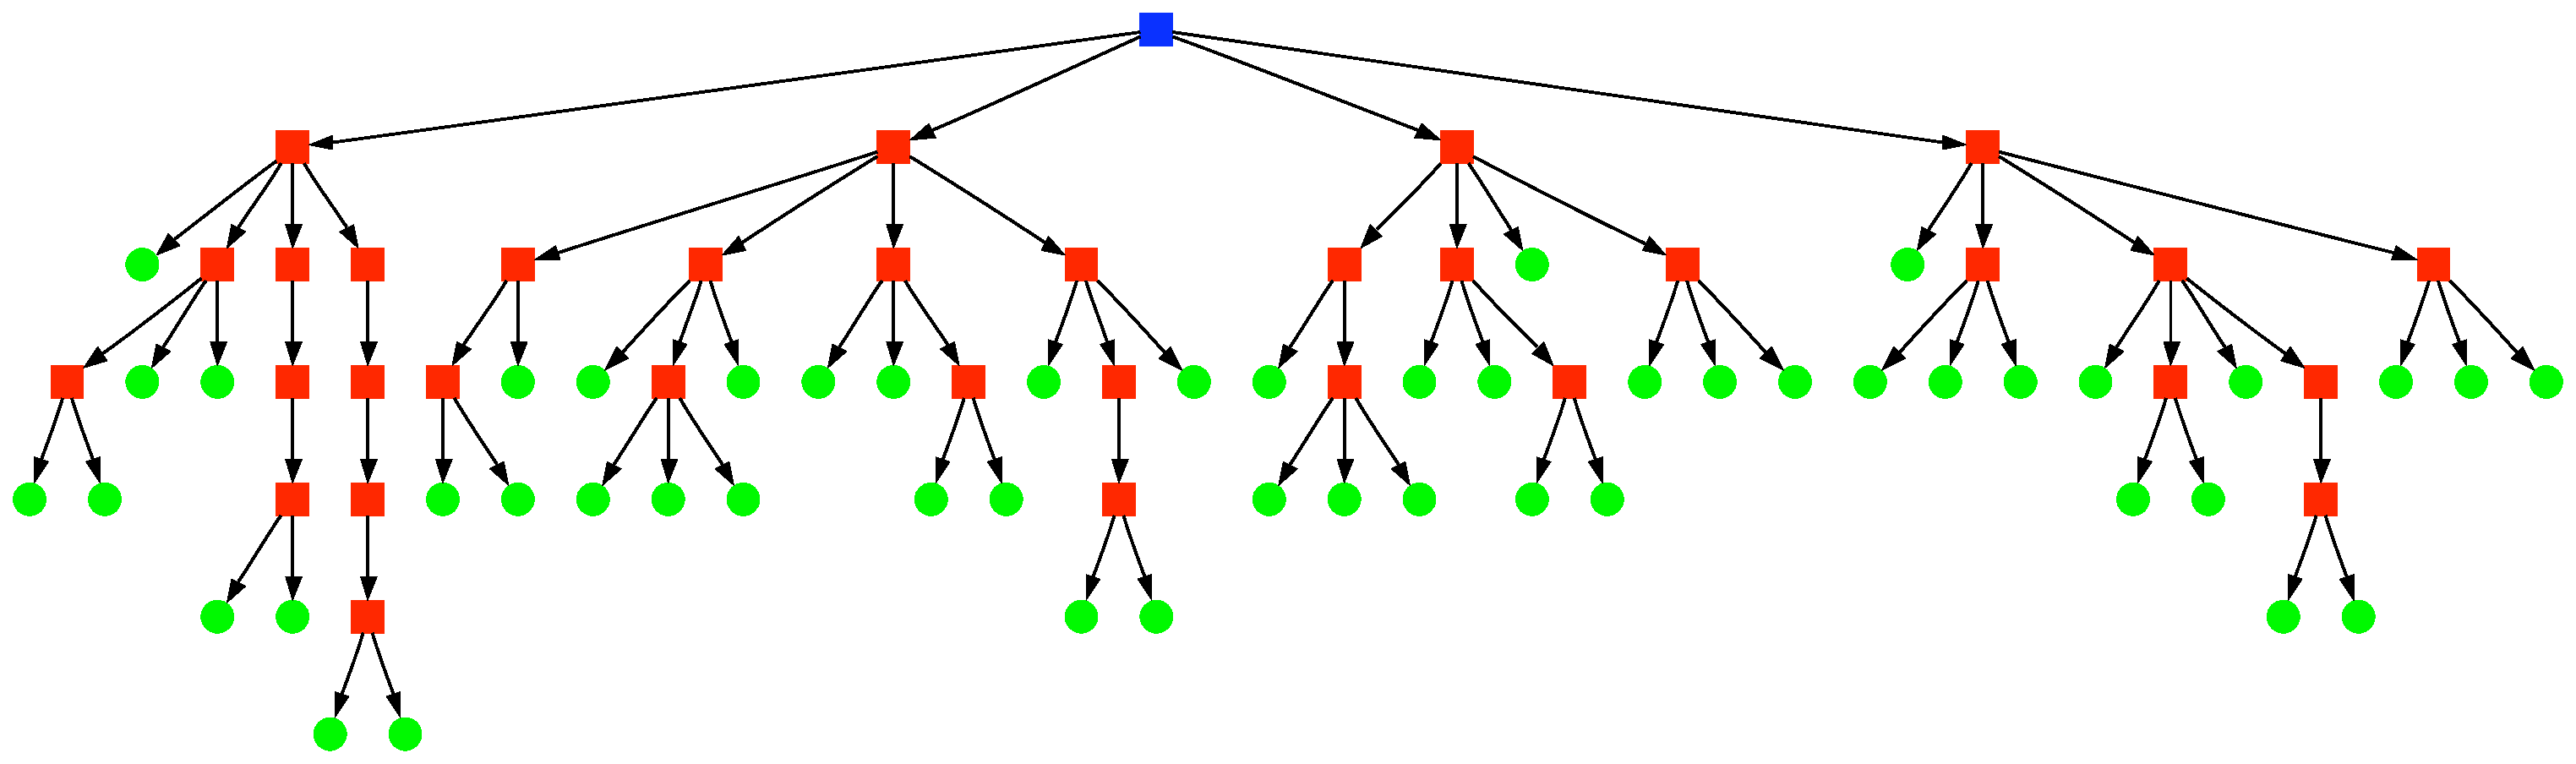
\includegraphics[scale=0.3]{quadtree50.pdf}
\caption{50 particles randomly distributed in $2D$ and the partitioning into cells (upper plot) with the and the corresponding \emph{quadtree} (lower plot)}
\label{fig:2D_BHtree}
\end{center}
\end{figure}



\begin{figure}[htbp]
\begin{center}

\includegraphics{ttnode_filled_local.pdf}

\includegraphics{ttnode_empty_local.pdf}

\includegraphics{node_filled_local.pdf}

\includegraphics{node_filled_remote.pdf}
\hspace{1cm}

\includegraphics{particle_filled_local.pdf}

\includegraphics{particle_filled_remote.pdf}
\caption{Symbols used for tree nodes. Squares stand for \emph{cells}, circles for \emph{particles}}
\label{fig:nodetypes}
\end{center}
\end{figure}


Each cell in the tree represents now a clump of particles. 

$\theta$ clumping parameter, self-acceleration for $\theta \ge 1$
